\section{Introduction}
Optimal Transport (OT) is well known for its many applications in various domains, especially when working in spaces of probability distributions. It has recently had major successes when applied to several machine learning problems in Computer Vision \cite{arjovsky_wasserstein_2017, rubner_earth_2000} or Natural Language Processing \cite{kusner_word_2015}. Although efficient ways of solving OT problems exist and are widely used in practice, they are impractical for very large scale settings, which creates the need for more efficient methods. 
Stochastic optimization is also an essential tool at the basis of numerous successes of machine learning and its immense developments. They allow to solve very large scale problem with reasonable time and memory requirements, which make them ideal for cases where traditional methods for solving OT problems fail. 

\subsection{Optimal transport : problem formulations}

Optimal transport dates back to 1781, when Monge studied the mathematical properties of problems involving the displacement of earth \cite{monge1781}. The problem has been first formulated in its modern form by Kantorovitch \cite{kantorovitch_on_1942}, allowing for continuous displacement of mass. OT can be interpreted as a way of defining a metric among probability distributions, called the \emph{Wasserstein} of \emph{earth mover's} distance. It is often described as a natural way to leverage the geometry of a space and define a metric on probability distributions, by opposition to the Euclidean distance and Kullback-Leibler divergence. 

\subsubsection{Entropic regularization of OT}
We consider two measures $\mu \in \mathcal{M}_+^1(\mathcal{X})$ and $\nu \in \mathcal{M}_+^1(\mathcal{Y})$ defined on metric spaces $\mathcal{X}$ and $\mathcal{Y}$. The cost of moving a unit of mass from $x\in \mathcal{X}$ and  $y\in \mathcal{Y}$ is defined by the continuous function $c \in \mathcal{C}(\mathcal{X}, \mathcal{Y})$, and written $c(x, y)$.
We also define the set of joint probability measures on $\mathcal{X}\times\mathcal{Y}$
\[
\Pi(\mu, \nu) \triangleq \{\pi \in \mathcal{M}_+(\mathcal{X}\times \mathcal{Y}) ; \forall (A, B) \subset \mathcal{X}\times \mathcal{Y}, \pi(A, \mathcal{Y}) = \mu(A), \pi(\mathcal{X}, B) = \nu(B)\}
\]
The entropic regularized version of the OT problem \cite{cuturi_sinkhorn_2013} can be written as a single convex optimization problem in the following form: $\forall (\mu, \nu)  \in \mathcal{M}_+^1(\mathcal{X})\times\mathcal{M}_+^1(\mathcal{Y}),$
\[\tag{$\mathcal{P}_\varepsilon$}
\label{eq:primal}
W_\varepsilon(\mu, \nu) \triangleq \min_{\pi\in \Pi(\mu, \nu)} \int_{\mathcal{X}, \mathcal{Y}} c(x, y)\text{d} \pi(x, y) + \varepsilon\text{KL}(\pi|| \mu \otimes \nu)
\]
With $\text{KL}(\pi|| \mu \otimes \nu)$ corresponding to the Kullback-Leibler divergence between measures $\pi$ and  $\mu \otimes \nu$, defined by $\text{KL}(\pi|| \xi) \triangleq  \int_{\mathcal{X}, \mathcal{Y}} \left(\log(\frac{d\pi}{d\xi}(x, y) - 1\right)d\xi(x, y)$.

For $\varepsilon > 0$, the above problem is strongly convex. \eqref{eq:primal} is usually called the primal form of the regularized OT problem, by opposition to the dual and semi-dual form that will be studied further.

\paragraph{Sinkhorn for discrete OT}
In the discrete setting $\mu = \sum_i^n\delta_{x_i}\bm{\mu}_i$ and $\nu = \sum_j^m\delta_{x_j}\bm{\nu}_j$, the sums are finite and the cost is $\mathbf{C} \in \mathbb{R}^{n\times m}$. The structure of the KL divergence gives the optimal solution $\mathbf{P}_\varepsilon \in \Pi(\mu, \nu)$ a convenient structure that makes it possible solving the problem using Sinkhorn's algorithm \cite{cuturi_sinkhorn_2013}. There indeed exist two scaling variables $\mathbf{u}_\varepsilon \in \mathbb{R}^n$ and $\mathbf{v}_\varepsilon \in \mathbb{R}^m$ such that
\[
\mathbf{P}_\varepsilon = \text{diag}(\mathbf{u}_\varepsilon)\mathbf{K}_\varepsilon\text{diag}(\mathbf{v}_\varepsilon)
\]
Where $(\mathbf{K}_\varepsilon)_{i,j} = \exp(-\mathbf{C}_{i,j}/\varepsilon)$ \cite{peyre_computational_2018}. Those scaling variables can be computed iteratively with the following update at step $\ell$,
\begin{gather}
\mathbf{u}^{\ell+1}_\varepsilon \triangleq \dfrac{\mu}{\mathbf{K}_\varepsilon\mathbf{v}^\ell_\varepsilon} \hspace{10pt}  \text{and} \hspace{10pt}\mathbf{v}^{\ell+1}_\varepsilon \triangleq \dfrac{\nu}{\mathbf{K}^T_\varepsilon\mathbf{u}^{\ell+1}_\varepsilon}
\end{gather}
Because each step of the algorithm relies on a vector-matrix computation, the overall complexity of the algorithm is $O(nm)$ in the most general configuration. Moreover, the rate of convergence of the algorithm is linear in the number of iterations \cite{franklin_scaling_1989}.

\begin{figure}[htb]
    \centering
    \begin{minipage}{.8\linewidth}
\begin{algorithm}[H]
    \caption{Sinkhorn algorithm}\label{alg:sinkhorn}
    \begin{algorithmic}[1]
        \State Data: $\mathbf{C}$, $\varepsilon$, $\mu$, $\nu$
        \State $\mathbf{K} \gets \exp(-\mathbf{C}/\varepsilon)$
        \State $\mathbf{u} = \mathbf{v} = 0$
        \While {!$(\texttt{stopping\_criterion})$} 
            \State $\mathbf{u} \gets \frac{\mu}{K\mathbf{v}}$
            \State $\mathbf{v} \gets \frac{\nu}{K^T\mathbf{u}}$
        \EndWhile
        \State \Return $\text{diag}(\mathbf{u})\mathbf{K}\text{diag}(\mathbf{v})$
    \end{algorithmic}
\end{algorithm}
\end{minipage}
\end{figure}


The algorithm can be used in a large scale setting by making use of specific hardware (multiple Wasserstein distances can be computed in parallel on a GPU \cite{slomp2011gpu}) and in some other specific cases where the kernel $\mathbf{K}$ is separable or can be expressed as a convolution \cite{peyre_computational_2018}. In the general case however, the computational complexity of Sinkhorn's algorithm can be prohibitively large for large scale problems.

The solution of an OT problem in the discrete setting can be represented as a transportation matrix $\mathbf{P}_\varepsilon$. An example of such a solution can be visualized along with two randomly generated measures on ${1, ..., 50}$ on Figure \ref{fig:example_discrete}. The distance matrix is the $L_2$ distance on the set ${1, ..., 50}$, the value of $\varepsilon$ was set to 1e-4 and the problem was solved with Sinkhorn's algorithm.

\begin{figure}[h]
    \centering
    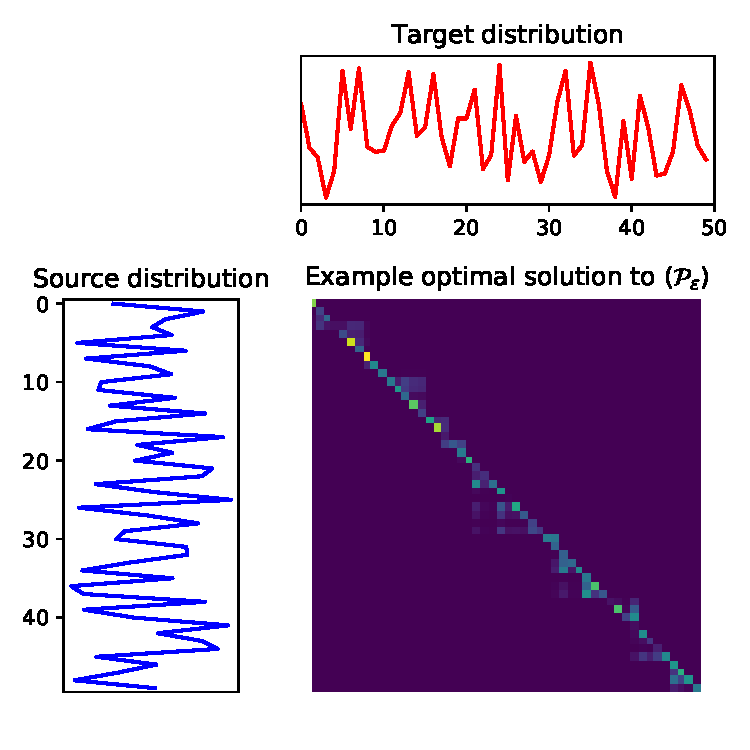
\includegraphics[width=0.4\linewidth]{figures/example_discrete.pdf}
    \caption{An example solution to discrete regularized OT for the \emph{blue} and \emph{red} discrete measures.}
    \label{fig:example_discrete}
\end{figure}

Naturally, most of the transport is concentrated close to the diagonal of the matrix, that is where the cost is smallest in the example.

\subsubsection{Dual and Semi-dual formulations}
The dual and semi-dual variations of the OT problem are essential for constructing and applying stochastic optimization methods to solve it.

We define the following set for $c\in \mathcal{C}(\mathcal{X}\times \mathcal{Y})$
\begin{align*}
    U_c \triangleq \left\{ (u, v) \in \mathcal{C}(\mathcal{X})\times \mathcal{C}(\mathcal{X}) ; \forall (x, y) \in \mathcal{X}\times\mathcal{Y}, u(x)+v(y) \leq c(x,y)\right\}
\end{align*}
The dual problem can be derived using Fencher-Rockafellar's theorem \cite{genevay_stochastic_2016} and reads
\begin{align*} 
    \label{eq:dual}
    \tag{$\mathcal{D_\varepsilon}$}
    W_\varepsilon(\mu, \nu) = \max_{(u, v)\in \mathcal{C}(\mathcal{X})\times\mathcal{C}(\mathcal{Y})} \int_\mathcal{X} u(x)\text{d}\mu(x) + \int_\mathcal{Y}v(y)\text{d}\nu(y) - \iota_{U_c}^\varepsilon(u, v)
\end{align*}
Where we have defined $\iota_{U_c}^0 = \iota_{U_c}$ and for $\varepsilon>0$, $\iota_{U_c}^\varepsilon$ is the \emph{smoothed} approximation of the indicator function of $U_c$,
\begin{align*}
    \iota_{U_c}^\varepsilon(u, v) = \varepsilon \int_{\mathcal{X}\times\mathcal{Y}} \exp\left(\dfrac{u(x)+v(y) - c(x, y)}{\varepsilon}\right)\text{d}\mu(x)\text{d}\nu(y)
\end{align*}
If we write the optimality conditions in $v$ of \eqref{eq:dual}, we get the following relation between $u$ and $v$
\begin{align*}
    \forall x \in \mathcal{X}, u(x) = v^{c, \varepsilon}(x) \triangleq \begin{cases}
        \min_{y\in \mathcal{Y}} c(x, y) - v(y) \hspace{10pt} \text{if } \varepsilon = 0\\
        -\varepsilon\log\left( \int_\mathcal{Y}\exp\left( \dfrac{v(y) - c(x, y)}{\varepsilon}\right) \right) \hspace{10pt} \text{if } \varepsilon > 0
    \end{cases}
\end{align*}
$v^{c, \varepsilon}$ is sometimes called the $c$-transform \cite{smooth_cuturi_peyre_2016} of dual variable $v$. By plugging this expression back into \eqref{eq:dual}, we get the semi-dual form of the OT problem
\begin{align*} 
    \label{eq:semi-dual}
    \tag{$\mathcal{S_\varepsilon}$}
    W_\varepsilon(\mu, \nu) = \max_{v\in\mathcal{C}(\mathcal{Y})} H_\varepsilon(v)\triangleq \int_\mathcal{X} v^{c,\varepsilon}(x)\text{d}\mu(x) + \int_\mathcal{Y}v(y)\text{d}\nu(y) - \varepsilon
\end{align*}
This formulation is crucial to solving the semi-discrete OT problem, because optimization can be done with respect to the discrete dual variable instead of the continuous one. 

\paragraph{Dual variables and Sinkhorn algorithm}
In the discrete setting, the scaling variables $\mathbf{u}$ and $\mathbf{v}$ of the Sinkhorn algorithm can be linked to the dual variables $u$ and $v$ of \eqref{eq:dual} with the relation 
\begin{align*}
    (\mathbf{u}, \mathbf{v}) = (\exp(u/\varepsilon), \exp(v/\varepsilon))
\end{align*}
The proof of this result can be found in \cite{peyre_computational_2018}. With these variables, the Sinkhorn algorithm can be re-written as a \emph{block coordinate ascent} strategy on the dual variables. 

We also note that, since the scaling variables of the Sinkhorn algorithm are defined up to a multiplicative constant $\lambda > 0$, the dual variables are also defined up to an additive constant. 

Furthermore, for a $v$ solving \eqref{eq:semi-dual}, an optimal $u$ can be recovered with $u = v^{c, \varepsilon}$ (this also shows that $u$ and $v$ can be translated by an arbitrary constant in opposite directions).
From a pair $(u,v)$ solving \eqref{eq:dual}, an optimal solution $\pi$ of \eqref{eq:primal} can be computed with $\text{d}\pi(x,y) = \exp\left(\frac{u(x) + v(y) - c(x, y)}{\varepsilon}\right)\text{d}\mu(x)\text{d}\nu(y)$.

\subsection{Relevant Work}
The unregularized Kantorovitch formulation \cite{kantorovitch_on_1942} of optimal transport is usually solved as a large scale linear program in the case of finite distributions (for example a network simplex algorithm). Some heuristics were introduced to cope with the relatively high computational cost of those method, such as pruning the long distances between histogram bins \cite{pele_fast_2009} or using quad-trees and random shifts such as in \cite{sharathkumar_near_linear_2012}.

Since the regularized version of the problem is strongly convex, it can benefit from all the optimization methods associated with and advantages of this property. As presented above, regularized optimal transport problems are usually tackled with Sinkhorn's algorithm \cite{cuturi_sinkhorn_2013}. Its linear convergence rate and paralellisation properties (showcased in \cite{solomon_convolutional_2015}) make it the prevalent way of computing solutions to the problem. 

For semi-discrete OT, the main way to compute solution to the problem is by using semi-discrete solvers such as \cite{aurenhammer_minkowski-type_1998}.

The implementations and stochastic formulations of discrete and semi-discrete optimal transport problems are based on Genevay et al.'s paper on stochastic optimization applied to optimal transport \cite{genevay_stochastic_2016}. This paper also explores the continuous-continuous setting, which has comparatively to the other two been less explored in practice because it involves estimating functions, which is a harder task in general. \cite{genevay_stochastic_2016} uses a Kernel expansion of the dual variables to solve the continuous-continuous problem, while \cite{arjovsky_wasserstein_2017} and \cite{seguy_large-scale_2017} have used neural networks to represent the dual variables.

\subsection{Contributions}
This contributions of this paper are the following: 
\begin{itemize}
    \item Lay out the stochastic formulations of discrete and semi-discrete OT problems proposed in \cite{genevay_stochastic_2016}.
    \item Implement and benchmark the SAG (Stochastic Average Gradient) algorithm \cite{schmidt_minimizing_2013} in the discrete setting on synthetic and real data, give some supplementary results to \cite{genevay_stochastic_2016}.
    \item Implement and benchmark the SAGA algorithm \cite{defazio_saga:_2014} in the same setting and compare its performances with SAG.
    \item Implement and benchmark the SGD algorithm for semi-discrete optimal transport on a socio-economic case study.
\end{itemize}
We show that stochastic optimization is a very useful tool for dealing with OT problems, as it provides a possibly more efficient way to compute solutions in a discrete setting and a general way of solving semi-discrete OT problems.
